\documentclass[ignorenonframetext,]{beamer}

%Set up notes
\setbeamertemplate{note page}[plain]
\setbeameroption{hide notes}

\usepackage{amssymb,amsmath}
\usepackage{ifxetex,ifluatex}
\usepackage{fixltx2e} % provides \textsubscript
\usepackage{tikz}
\usepackage{tikz-qtree}
\usepackage{pdfpages} %include beamer pdf slides from other presentations
\ifxetex
  \usepackage{fontspec,xltxtra,xunicode}
  \defaultfontfeatures{Mapping=tex-text,Scale=MatchLowercase}
\else
  \ifluatex
    \usepackage{fontspec}
    \defaultfontfeatures{Mapping=tex-text,Scale=MatchLowercase}
  \else
    \usepackage[utf8]{inputenc}
  \fi
\fi

% Comment these out if you don't want a slide with just the
% part/section/subsection/subsubsection title:
\AtBeginPart{
  \let\insertpartnumber\relax
  \let\partname\relax
  \frame{\partpage}
}
\AtBeginSection{
  \let\insertsectionnumber\relax
  \let\sectionname\relax
  \frame{\sectionpage}
}
\AtBeginSubsection{
  \let\insertsubsectionnumber\relax
  \let\subsectionname\relax
  \frame{\subsectionpage}
}

\setlength{\parindent}{0pt}
\setlength{\parskip}{6pt plus 2pt minus 1pt}
\setlength{\emergencystretch}{3em}  % prevent overfull lines
\setcounter{secnumdepth}{0}

\title{Inequality and Trade: The Specific Factors Model}
\author{Instructor: David Jinkins}
\date{Date: Sept. 9, 2014}

\begin{document}

\frame{\titlepage}

\begin{frame}
\begin{itemize}
\itemsep1pt\parskip0pt\parsep0pt
\item
  Last week

  \begin{itemize}
  \itemsep1pt\parskip0pt\parsep0pt
  \item Gravity model:
      \begin{enumerate}
          \item Derivation
          \item Country-specific constant: remoteness
      \end{enumerate}
  \item Ricardian model:
      \begin{enumerate}
          \item Equilibrium wages different across countries
          \item Labor migration determined by absolute advantage
          \item Data: Countries export in relatively productive industries 
          \item Institutions such as trust may cause differences in technology
      \end{enumerate}
  \end{itemize}
\end{itemize}

\end{frame}

\begin{frame}
\begin{itemize}
\itemsep1pt\parskip0pt\parsep0pt
\item
  Today: Effect of trade on income distributions
  \begin{itemize}
        \item Specific factors Model
        \begin{itemize}
            \item Definition of specific factor
            \item Simplest possible model
            \item Production potential
            \item Autarchy equilibrium and comparative statics
            \item Trade equilibrium/Gains from Trade
        \end{itemize}
        \item Political economy: a preview
        \item Labor migration
        \begin{itemize}
            \item Theory
            \item Evidence
        \end{itemize}
    \end{itemize}
\end{itemize}

\end{frame}

\begin{frame}{Ricardo Redux}

    \begin{itemize}
        \item Reason for trade: technological differences (comp. adv.)
        \item All countries \emph{weakly} gain from trade
        \item All income goes to labor $/rightarrow$ all workers gain
        \item Since everyone the same, income distribution is degenerate
    \end{itemize}

\end{frame}

\begin{frame}{Sometimes trade hurts}

    \begin{itemize}
        \item Why might trade liberalization hurt some?
        \begin{itemize}
            \item Short run: adjustment costs like training or refitting machinery
            \item Long run: some inputs no longer needed as much
            \item Long run example from book: Japanese rice farming machinery 
        \end{itemize}
    \end{itemize}

\end{frame}

\begin{frame}{Specific factors}

    \begin{itemize}
        \item Today: Focus on the short run
        \begin{itemize}
            \item \emph{Specific factors} can only be used to make one good
            \item Ex: Try to open a restaurant using a car manufacturing plant
            \item Given enough time\dots
        \end{itemize}
        \item Evidence: American ``displaced'' workers suffer permanent 15\% (avg.) drop in wages 
    \end{itemize}

\end{frame}

\begin{frame}{Specific factors}

    \begin{itemize}
        \item Why do countries trade? 
        \begin{itemize}
            \item Unlike Ricardo: same technology in all countries 
            \item Countries have different factor mix (more or less capital, say)
            \item Different factor mix causes countries to specialize
            \item Ex: More capital makes cars, more labor makes textiles
        \end{itemize}
    \end{itemize}

\end{frame}

\begin{frame}{Simplest possible model for income distributions}

    \begin{itemize}
        \item Two countries: Home (H) and Foreign (G)
        \item Two goods: Clothes (C) and Food (F)
        \item \emph{Two} factors: Land (t) and Capital (k)
        \item Different from textbook (three factors)!
        \item Home endowment of land $T$ less than foreign $T^*$
        \item Home endowment of capital $K$ greater than foreign $K^*$
    \end{itemize}

\end{frame}

\begin{frame}{Two factor model}

    \begin{itemize}
        \item Specific factors
        \begin{itemize}
            \item Income dist.: different people own Land and Capital 
            \item Capital is used \emph{only} to make clothes
            \item Land is used \emph{only} to make food
        \end{itemize}
        \item Production technology
        \begin{itemize}
            \item Clothes: $f_C(k) = \frac{k}{a_C}$
            \item Food: $f_F(t) = \frac{t}{a_F}$
            \item Same technology in both countries
        \end{itemize}
    \end{itemize}

\end{frame}

\begin{frame}{Production Possibilities Sets}

\end{frame}

\begin{frame}{Payments to factor owners}

    \begin{itemize}
        \item Like wages last time 
        \item Capital gets $r_k = \frac{P_C}{a_C}$
        \item Land gets $r_t = \frac{P_F}{a_F}$
    \end{itemize}

\end{frame}

\begin{frame}{Equilibrium prices}

    \begin{itemize}
        \item As last time, relative demand and supply
    \end{itemize}

\end{frame}

\begin{frame}{Equilibrium Gains from Trade}

    \begin{itemize}
        \item autarchy home price ratio $< \frac{P_C^e}{P_F^e} <$ autarchy foreign price ratio
    \end{itemize}
    \begin{center}
        \begin{tabular}{llll}
            \hline \hline
                               & Input               & Clothes                            & Food \\ \hline
            Home capital owner & One unit of capital & $\frac{1}{a_C}$                    & $\frac{P^e_C}{P^e_F}\frac{1}{a_C}$ \\
            Home land owner    & One unit of land    & $\frac{P^e_F}{P^e_C}\frac{1}{a_F}$ & $\frac{1}{a_F}$  \\
            \hline
        \end{tabular}
    \end{center}
    \begin{itemize}
        \item Home capital owner gains from trade, but home land owner is hurt!
    \end{itemize}

\end{frame}

\begin{frame}{The textbook model}

    \begin{itemize}
        \item The textbook model adds to capital and land a \emph{mobile} factor called labor.  Why?
        \item Historical reason -- Paul Samuelson ``Ohlin was Right'', Swedish Journal of Economics 1971
        \item Ohlin: If technology is shared, factor prices ($r_k$, $r_t$, and $w$) equalize across countires if factors can move, but not if only goods are traded
        \item But factor prices do equalize if there are the same number of factors and goods
        \item Just now, for ex., equilibrium capital rent in both countries is $r_k = P^e_C / a_C$
    \end{itemize}

\end{frame}
    
\begin{frame}{The textbook model}

    \begin{itemize}
        \item Samuelson (and Ron Jones independently) developed the textbook version
        \item Countries with different endowments of land and capital can end up with different factor prices
        \item Point is to study \emph{how} and \emph{why} factor prices differ across countries
        \item Desirable, because in the real world wages and other factor prices widely differ
        \item Of course, analysis a bit more complicated
    \end{itemize}

\end{frame}

\begin{frame}{Production technology}

    \begin{itemize}
        \item Clothing
        \begin{itemize}
            \item In two factor example, production function $f(k) = \frac{k}{a_c}$
            \item Now production function for clothing $f(k,l)$
            \item Textbook notation $Q_C(K,L_C)$
        \end{itemize}
        \item Food
        \begin{itemize}
            \item In two factor example, production function $f(t) = \frac{t}{a_f}$
            \item Now production function for clothing $f(t,l)$
            \item Textbook notation $Q_F(T,L_F)$
        \end{itemize}
    \end{itemize}

\end{frame}

\begin{frame}{Production function}

    \begin{itemize}
        \item Clothing, fix capital at $K$
    \end{itemize}
    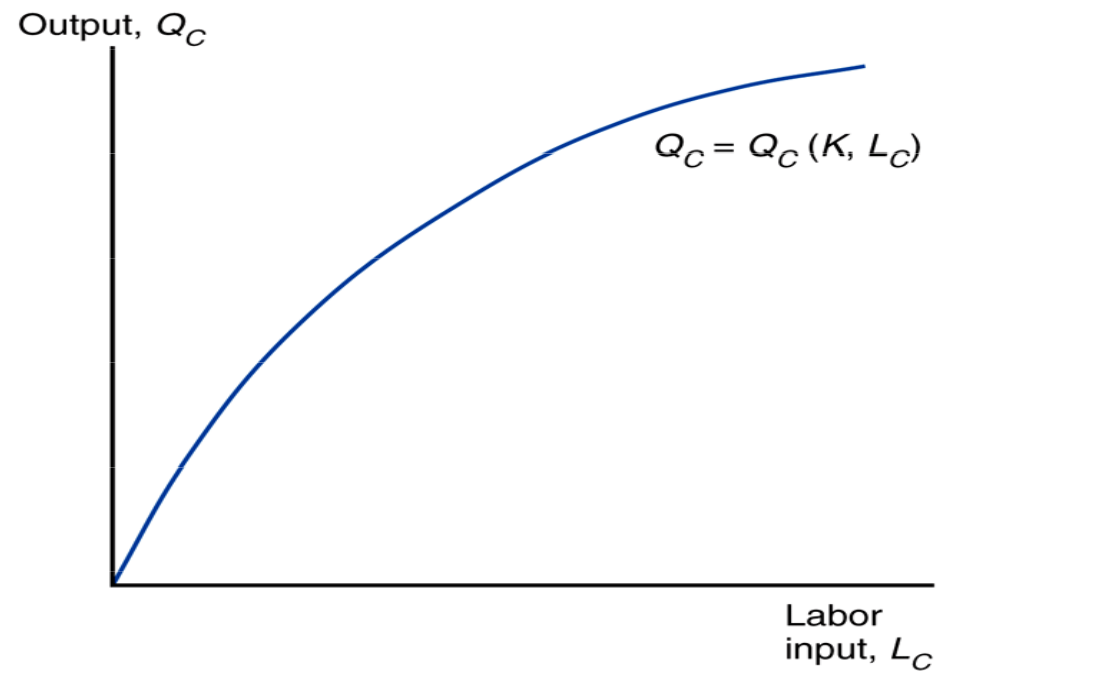
\includegraphics[scale=0.20]{cloth_prod.png}

\end{frame}

\begin{frame}{Decreasing MPL}

    \begin{itemize}
        \item Clothing, fix capital at $K$
    \end{itemize}
    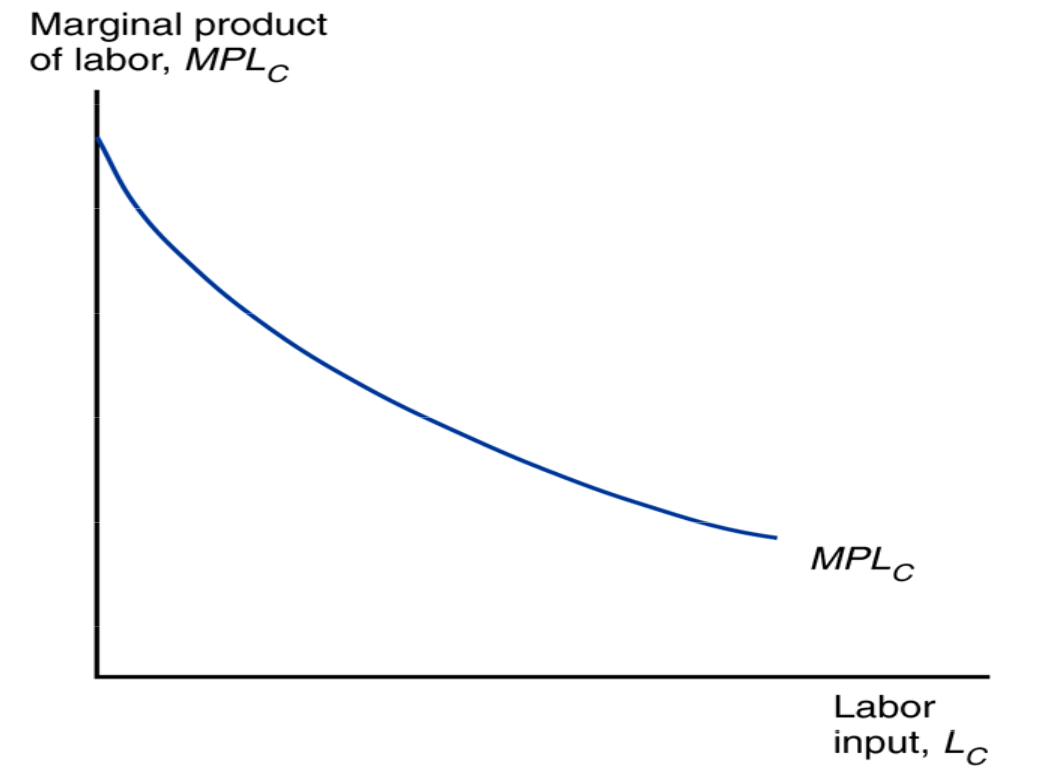
\includegraphics[scale=0.20]{cloth_mpl.png}

\end{frame}

\begin{frame}{Graphically deriving the PPF}

    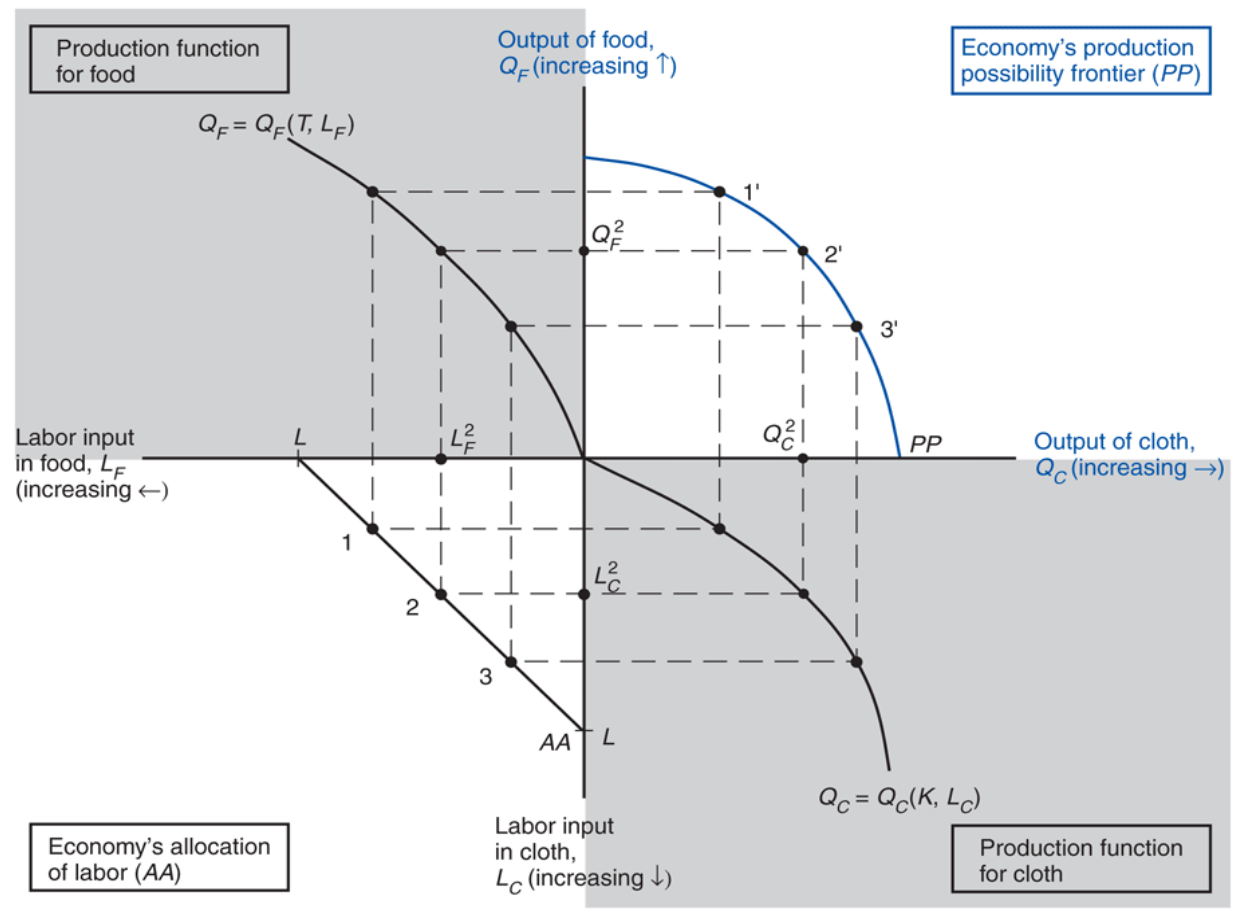
\includegraphics[scale=0.25]{ppf.png}

\end{frame}

\begin{frame}{Important PPF observation}

    \begin{itemize}
        \item The slope of the production possibilities frontier is $-\frac{Q^F_L(T,L_F)}{Q^C_L(K,L_C)}$
        \item Another way to write this: $-\frac{MPL_F}{MPL_C}$
        \item Heuristic argument -- how much food do I have to give up to get a bit more clothing?
    \end{itemize}

\end{frame}

\begin{frame}{Taking a step back}

    \begin{itemize}
        \item We have described what goods it is \emph{possible} for a country to produce
        \item EG, if you were the dictator what mix of goods could you order produced
        \item But what goods \emph{will} be produced by the economy in autarchy?
        \item What about with trade?
    \end{itemize}

\end{frame}

\begin{frame}{Autarchy wage}

    \begin{itemize}
        \item Competitive firms, zero profit
        \item Wage:
            \begin{equation*}
                w = Q^C_L(K,L_C) P_C = Q^F_L(T,L_F) P_F
            \end{equation*}
        \item Textbook equivalently writes:
            \begin{equation*}
                w = MPL_C P_C = MPL_F P_F 
            \end{equation*}
        \item Why do these equations hold?
        \item Last week:
            \begin{equation*}
                w = \frac{P_c}{a_c} = \frac{P_w}{a_w}
            \end{equation*}
    \end{itemize}

\end{frame}

\begin{frame}{Graphical Autarchy wage}

    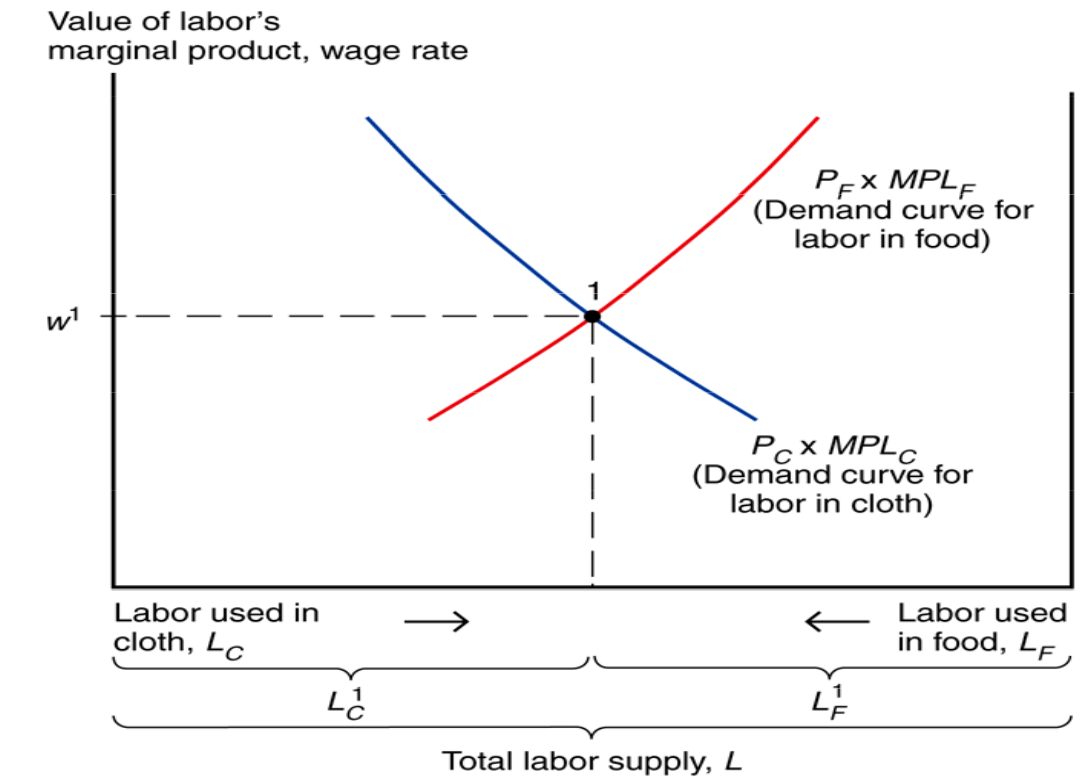
\includegraphics[scale=0.25]{aut_wage.png}

\end{frame}

\begin{frame}{Autarchy Equilibrium and the PPF}

    \begin{itemize}
        \item Wage given by:
            \begin{equation*}
                w = MPL_C P_C = MPL_F P_F 
            \end{equation*}
        \item We can write:
            \begin{equation*}
                -\frac{P_C}{P_F} = -\frac{MPL_F}{MPL_C}
            \end{equation*}
        \item Where have we seen the RHS?
    \end{itemize}

\end{frame}

\begin{frame}{Equilibrium and the PPF}

    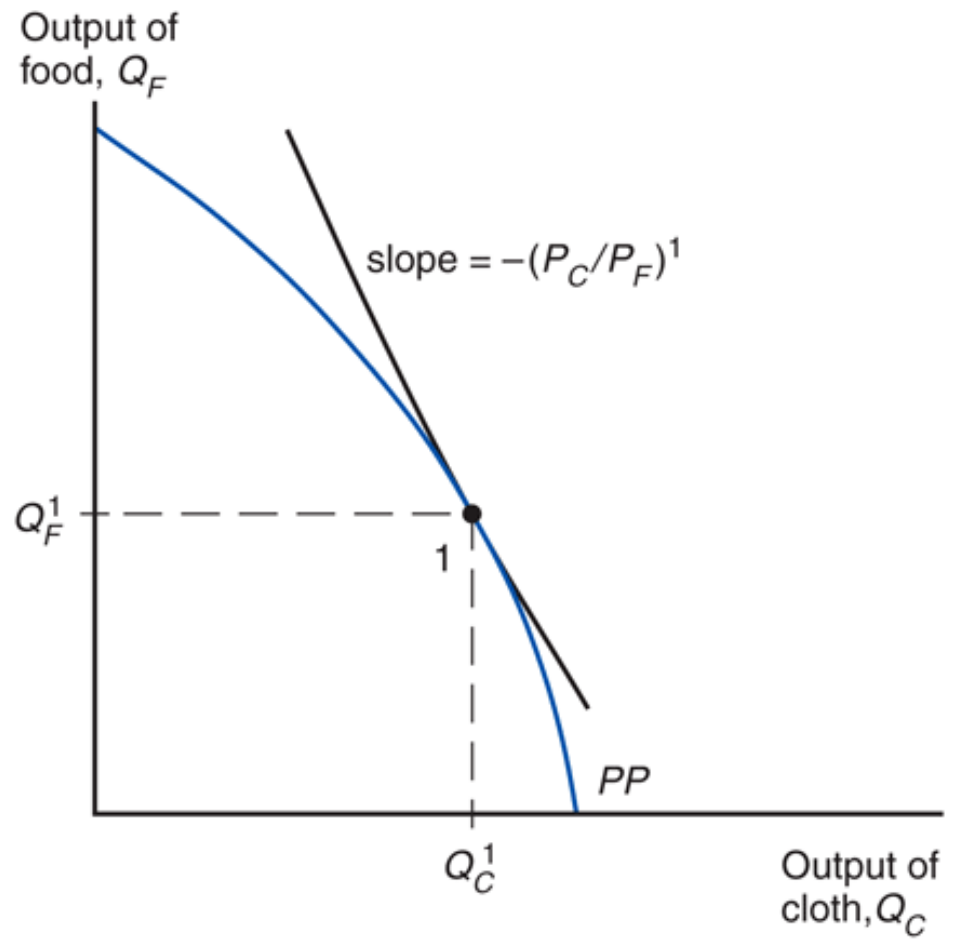
\includegraphics[scale=0.25]{ppf_equib.png}

\end{frame}

\begin{frame}{Price changes, labor allocation, and wages}

        \begin{itemize}
            \item Who is helped or hurt by:
            \begin{enumerate}
                \item Proportional rise in prices
                \item Change in relative prices 
            \end{enumerate}
            \item The book is hand-wavy here 
            \item We need to know:
            \begin{itemize}
                \item What is payment to capital?
                \item What is payment to land?
                \item What is payment to labor?
            \end{itemize}
        \end{itemize}

\end{frame}

\begin{frame}{Price changes, labor allocation, and wages}
    
    \begin{itemize}
        \item Proportional increase in wage, no labor allocation change 
    \end{itemize}

    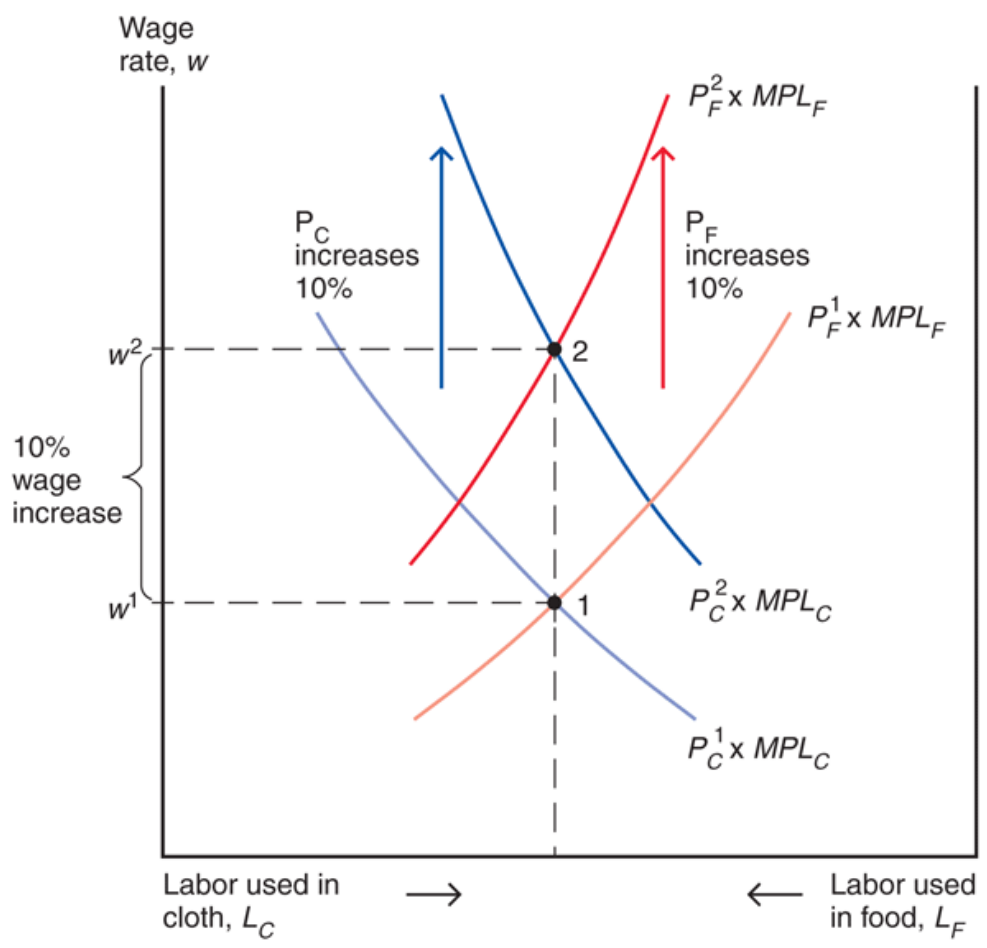
\includegraphics[scale=0.22]{prop_price_change.png}

\end{frame}

\begin{frame}{Price changes, labor allocation, and wages}

    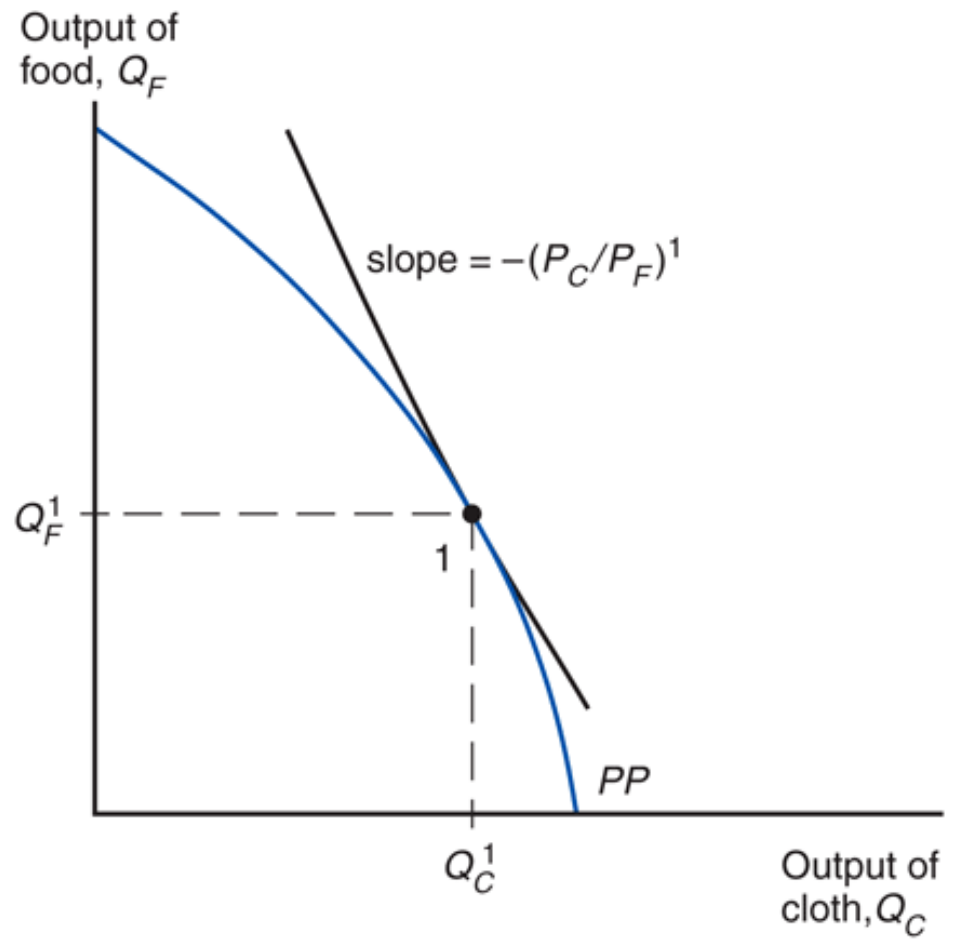
\includegraphics[scale=0.25]{ppf_equib.png}

\end{frame}

\begin{frame}{Price changes, labor allocation, and wages}

    \begin{itemize}
        \item Proportional price changes
        \begin{itemize}
            \item No one hurt, as all returns rise proportionally to price
        \end{itemize}
    \end{itemize}

\end{frame}

\begin{frame}{Price changes, labor allocation, and wages}
    \begin{itemize}
        \item Less than proportional increase in wage due to falling MPL 
    \end{itemize}

    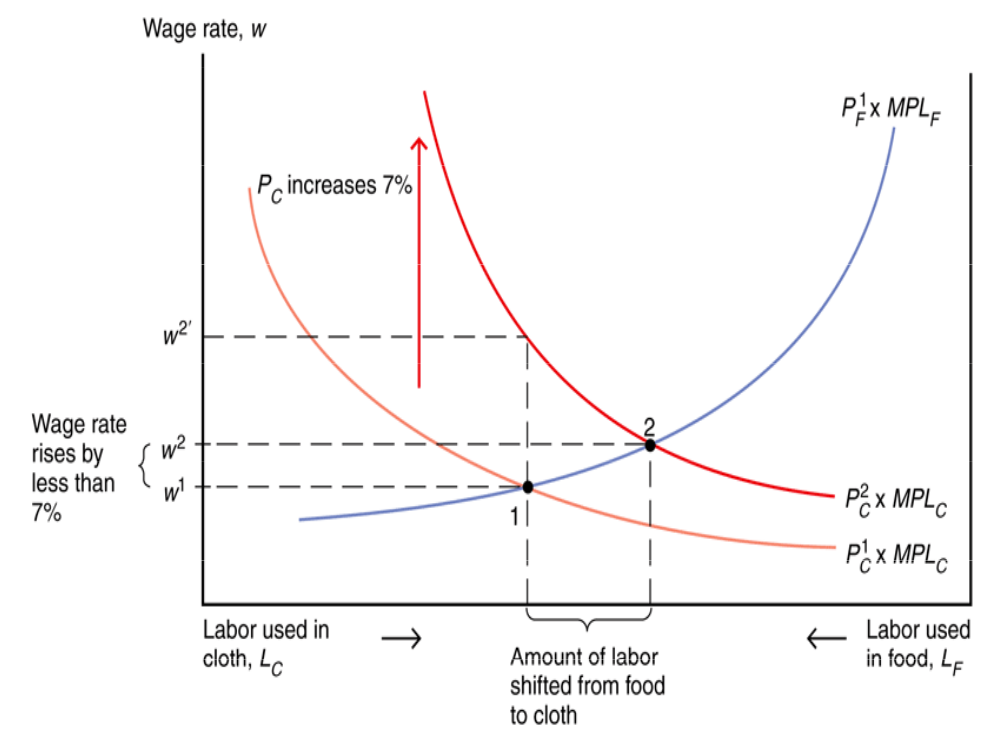
\includegraphics[scale=0.25]{rel_price_change.png}

\end{frame}

\begin{frame}{Price changes, labor allocation, and wages}

    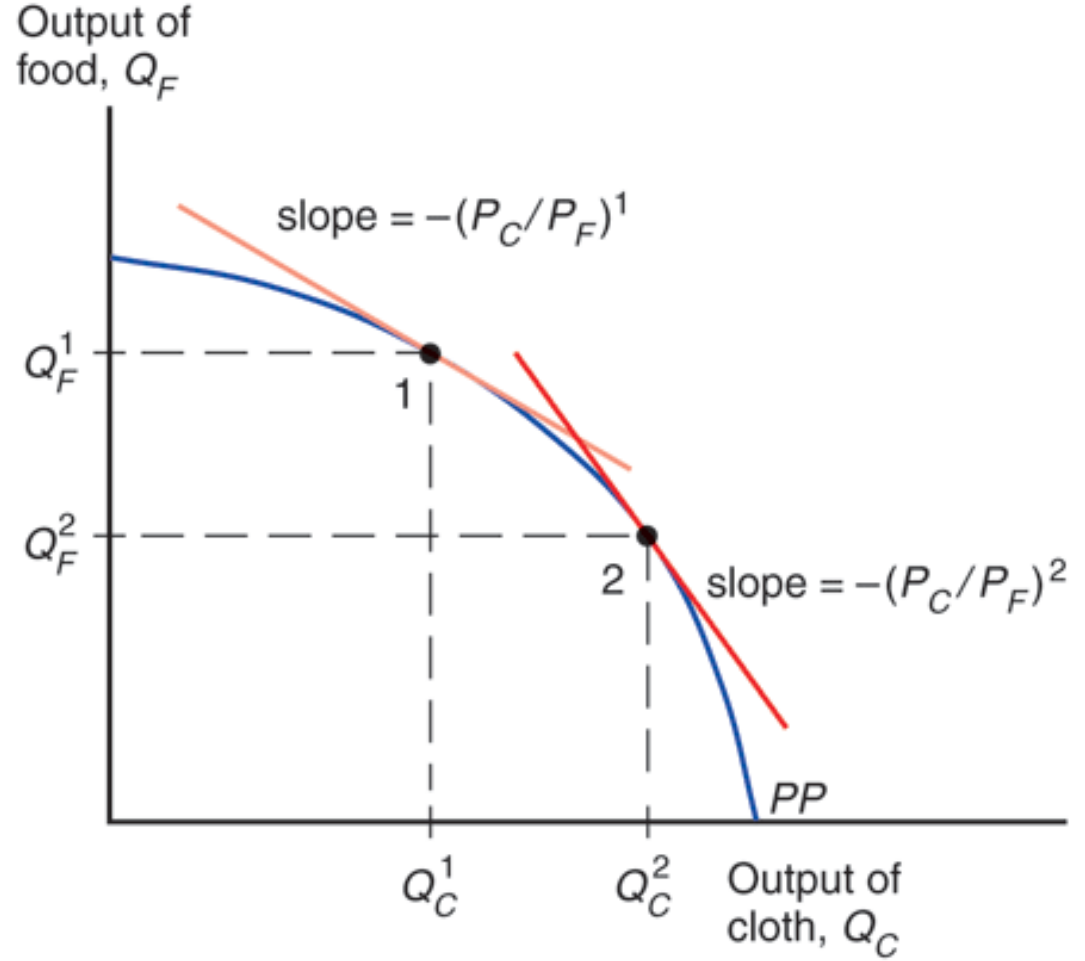
\includegraphics[scale=0.25]{rel_price_ppf.png}

\end{frame}

\begin{frame}{Price changes, labor allocation, and wages}

    \begin{itemize}
        \item Rise in price of clothes relative to food 
        \item Begin waving of hands
        \begin{itemize}
            \item Labor
            \begin{itemize}
                    \item Wage rises, but price of clothes rises more!
                    \item Workers can afford more food, but less clothes
                    \item Indeterminent effect on welfare
            \end{itemize}
            \item Capital
            \begin{itemize}
                    \item Price of clothes rises $\rightarrow$ pushes $r_k$ up.
                    \item What happens to the marginal product of capital when $L_c$ increases? 
                    \item Good reason to think that marginal product of capital should increase
                    \item However what if $Q_C(K,L_C) = (K-L)^2$?
            \end{itemize}
            \item Land 
            \begin{itemize}
                    \item Price of food stays constant, but clothes now more expensive! 
                    \item Textbook assumes that marginal product of land goes down as $L_F$ decreases 
                    \item Thus $r_t$ goes down, and price of clothes goes up, so land owners hurt.
            \end{itemize}
        \end{itemize}
    \end{itemize}

\end{frame}

\begin{frame}{Autarchy equilibrium rel quantities and prices}

    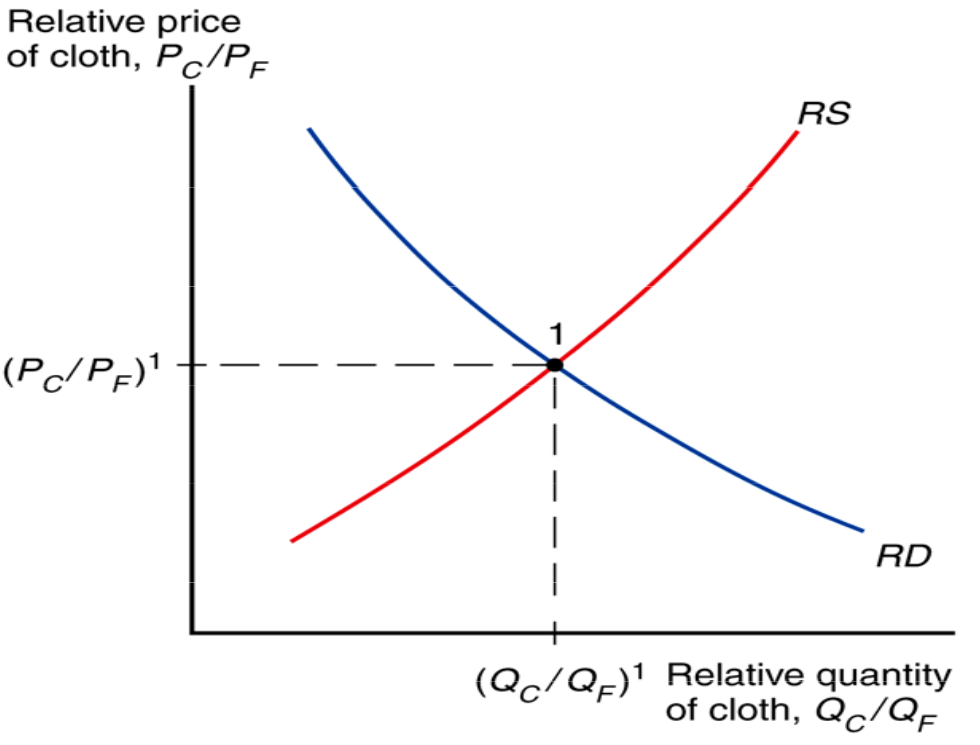
\includegraphics[scale=0.25]{aut_equib_rel.png}

\end{frame}

\begin{frame}{Trade equilibrium}

    \begin{itemize}
        \item We can think of opening up to trade as a change in relative prices, in one direction or the other
    \end{itemize}
        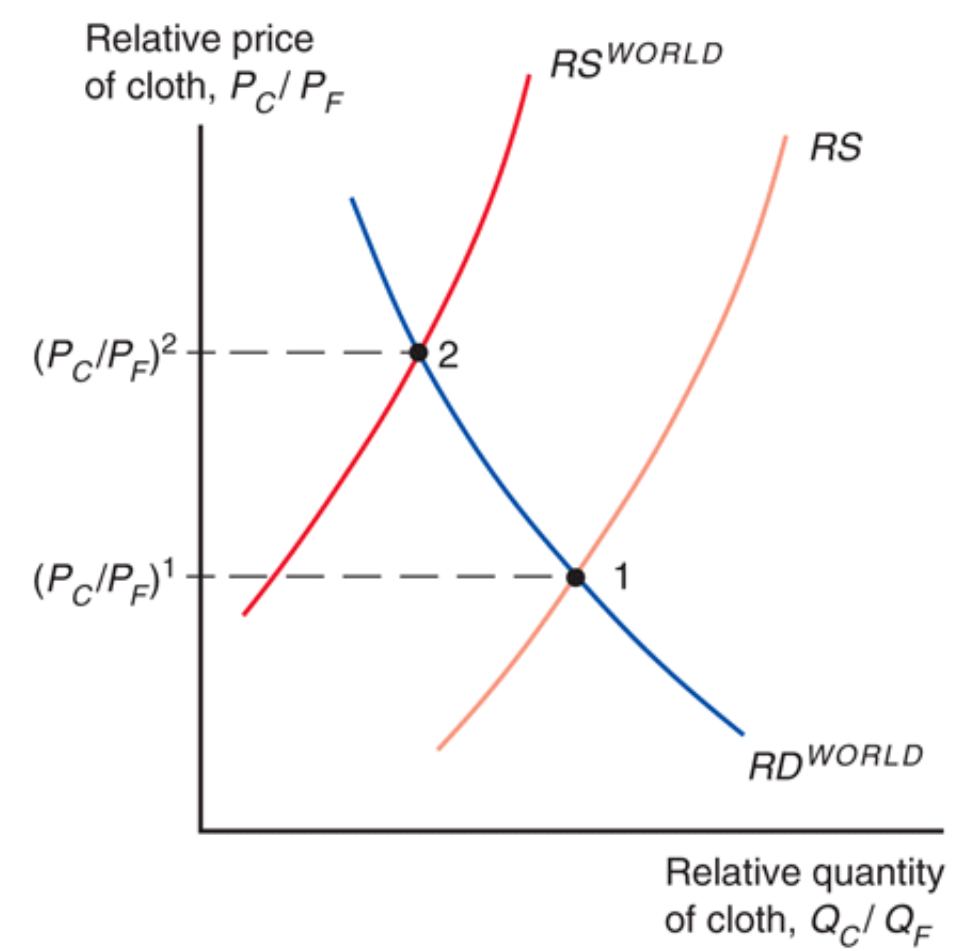
\includegraphics[scale=0.25]{trade_equil.png}

\end{frame}

\begin{frame}{Trade equilibrium}

    \begin{itemize}
        \item Since trade is just a relative price change, our autarchy intuition holds
        \item If price of clothes goes up, capital gains, land loses, and labor is indeterminant
    \end{itemize}

\end{frame}

\begin{frame}{Trade equilibrium}

    \begin{itemize}
        \item How can factor prices differ between countries?
        \item Final good prices ($P_C$ and $P_F$) in trade equilibrium are the same everywhere
        \item Consider two countries, same about of labor and land, but home has more capital.
        \item Wages are higher at home, returns to land are lower at home, and return to capital indeterminate
        \item If we don't have time $\rightarrow$ homework
    \end{itemize}

\end{frame}

\begin{frame}{Gains from Trade}

    \begin{itemize}
        \item Should countries restrict trade to prevent harm?
        \item Typically economists say no
        \item We will now show that with correct taxes and redistribution, trade can always make everyone better off
        \item Method: Show that trade expands the aggregate consumption possibilities set
    \end{itemize}

\end{frame}

\begin{frame}{Summing up}

    \begin{enumerate}
        \item Simple model shows how trade can hurt some within a country
        \item Textbook model shows how factor prices can differ in equilibrium, even if technology is the same
        \item Everyone can still gain from trade, with the right redistribution
    \end{enumerate}
    \begin{itemize}
        \item Now:
        \begin{itemize}
            \item Factor movement (international migration)
            \item Some evidence
        \end{itemize}
    \end{itemize}

\end{frame}

\begin{frame}{Note: Political economy}

    \begin{itemize}
        \item Trade can hurt: American apparel workers get 35\% lower wages than others
        \item We have shown, better to tax and distribute rather than stop trade
        \item Still politically much anti-trade rhetoric 
        \begin{itemize}
            \item Losses from trade are often concentrated in industries
            \item Gains are often distributed over many people 
        \end{itemize}
        \item Ex: American sugar twice as expensive as world sugar
        \item Half of American sugar production in 17 factories
        \item Costs avg. American \$10 (55 dkk) a year
    \end{itemize}

\end{frame}

\begin{frame}{International Migration}

    \begin{itemize}
        \item The single largest economic distortion in the world is barriers to migration
        \item The gains to opening borders are on the order of trillions of DKK a year
    \end{itemize}
    \begin{itemize}
        \item Textbook: Who gains and who loses in a simple model of international migration?
        \item The simplest possible model: 
        \begin{itemize}
            \item Two countries 
            \item One good: Cheese
            \item Two factors, labor and land
            \item Why do we need two factors?
        \end{itemize}
    \end{itemize}

\end{frame}

\begin{frame}{International Migration}

    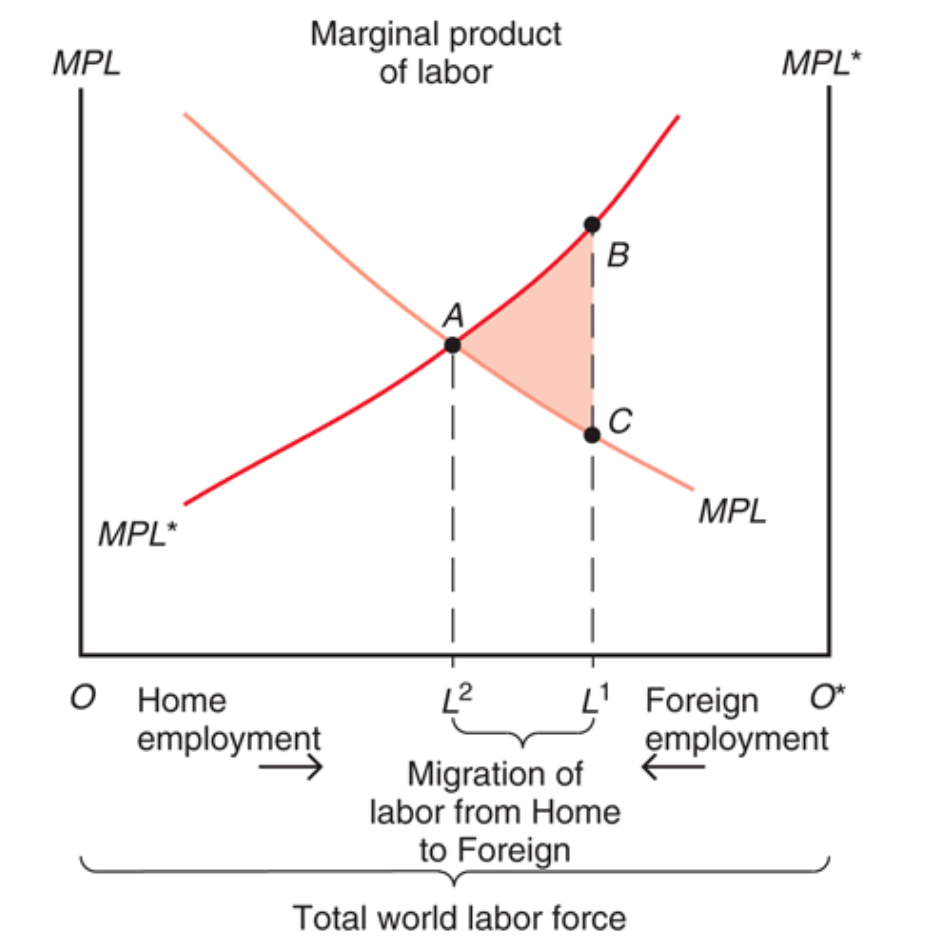
\includegraphics[scale=0.25]{labor_mig.png}

\end{frame}

\begin{frame}{International Migration}

    \begin{itemize}
        \item No price, only cheese
        \item Foreign workers lose 
        \item Home workers gain
        \item More cheese is produced, scope for welfare increasing taxes!
    \end{itemize}

\end{frame}

\begin{frame}{International Migration}

    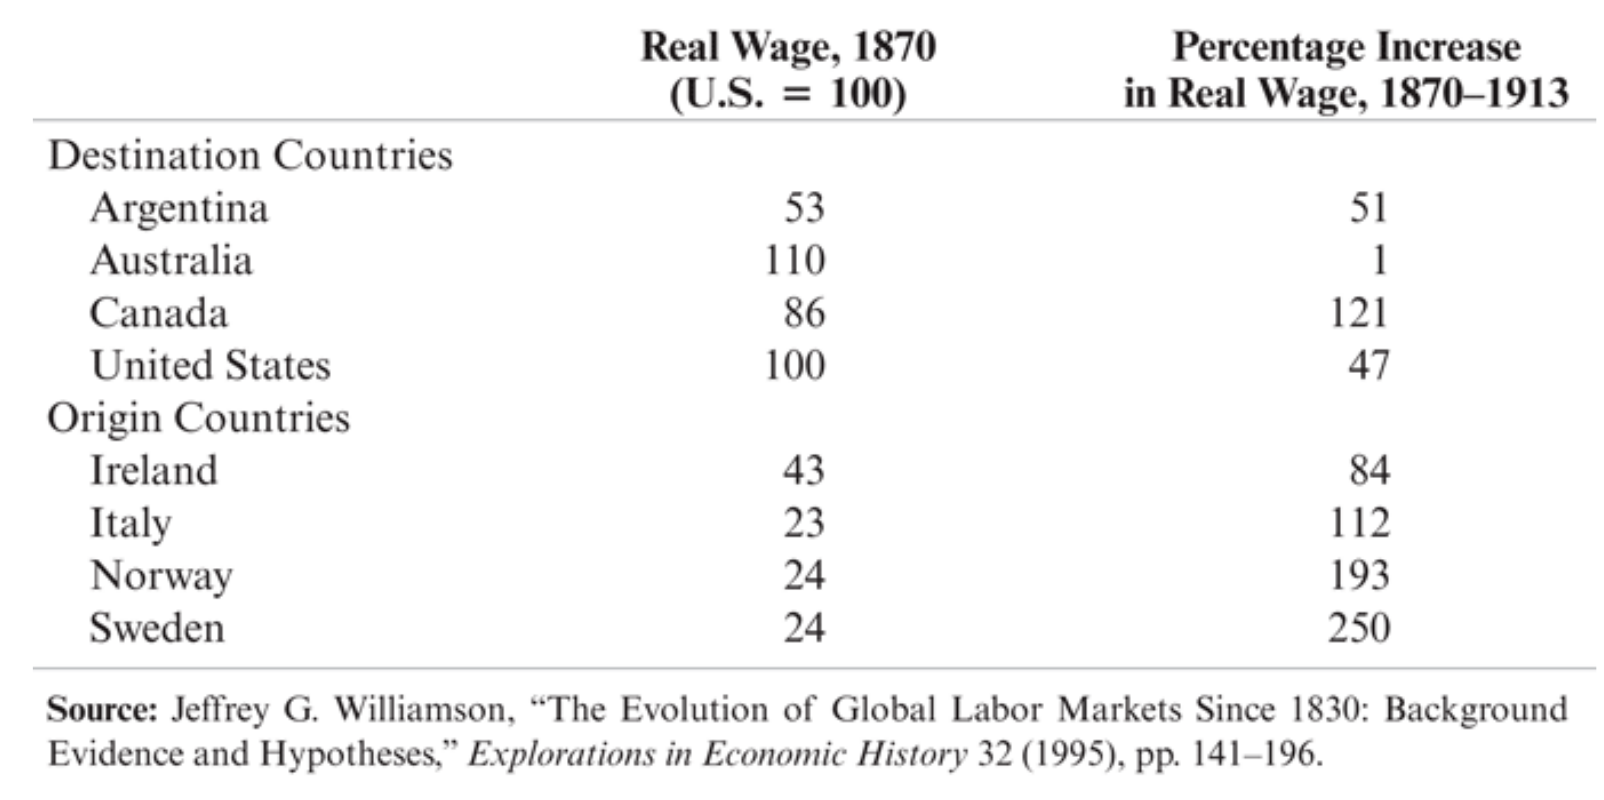
\includegraphics[scale=0.20]{migration_wages.png}

\end{frame}

\begin{frame}
\begin{itemize}
\itemsep1pt\parskip0pt\parsep0pt
\item
  Summary: Effect of trade on income distributions
  \begin{itemize}
        \item Specific factors Model
        \begin{itemize}
            \item Definition of specific factor
            \item Simplest possible model
            \item Production potential
            \item Autarchy equilibrium and comparative statics
            \item Trade equilibrium/Gains from Trade
        \end{itemize}
        \item Political economy: a preview
        \item Labor migration
        \begin{itemize}
            \item Theory
            \item Evidence
        \end{itemize}
    \end{itemize}
\end{itemize}

\end{frame}

\begin{frame}{Next time}

    \begin{itemize}
        \item The Hecksher-Ohlin Model
        \begin{itemize}
            \item Like model today, \emph{but} two mobile factors
            \item This was \emph{the} workhorse trade model for 50 years 
            \item Enough realism to examine many trade issues
            \item Why? My theory: can be almost totally analyzed graphically
        \end{itemize}
        \item Significant decline in popularity over last 20 years
        \begin{itemize}
            \item Great theory as it is testable!
            \item Unfortunately has spectacularly failed nearly 
            \item Still alive (barely)
        \end{itemize}
    \end{itemize}

\end{frame}

\frame[plain]{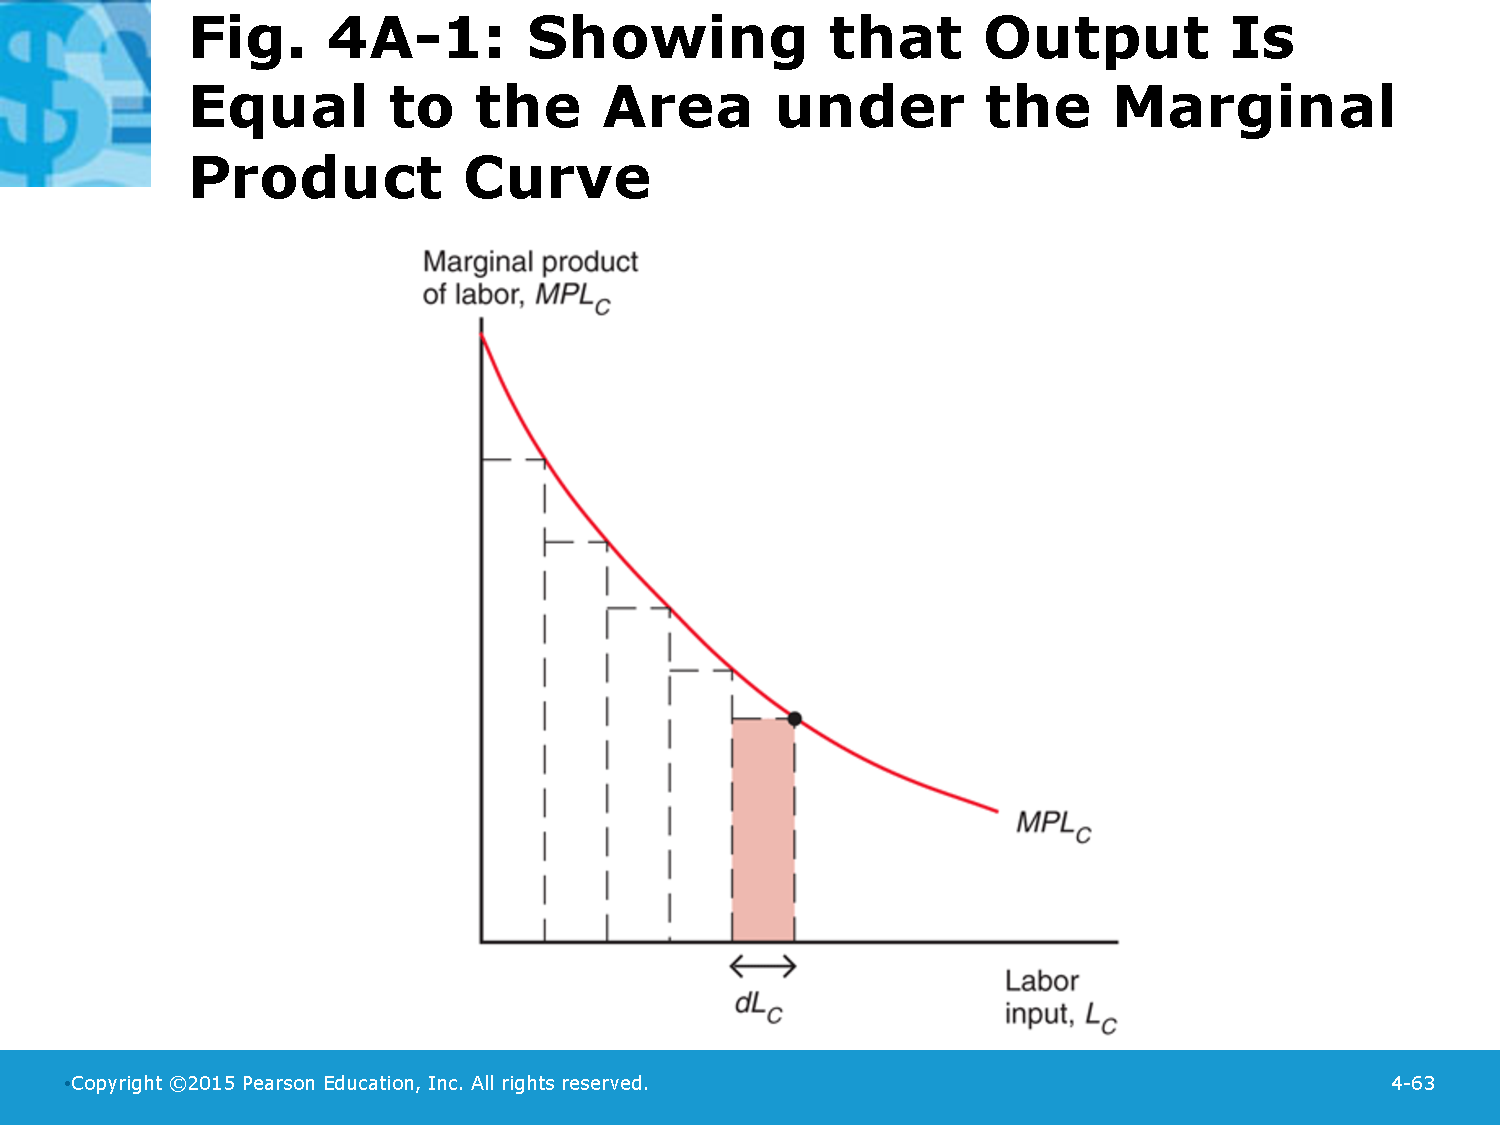
\includegraphics[page=1,width=\textwidth]{Pearson_math_appendix.pdf}}
\frame[plain]{\includegraphics[page=2,width=\textwidth]{Pearson_math_appendix.pdf}}
\frame[plain]{\includegraphics[page=3,width=\textwidth]{Pearson_math_appendix.pdf}}
\frame[plain]{\includegraphics[page=4,width=\textwidth]{Pearson_math_appendix.pdf}}

\end{document}




